\begin{spacing}{1.3}
    \section{Intro. to Heap}

    Omitting excessive introductions, now we want a data structure that supports 
    two operations:
    \begin{itemize}
        \item {\bf Insert}: insert a new element into it
        \item {\bf Extract-Min}: removes and returns the smallest element inside
    \end{itemize}

    For now, you may come up with some possible implementations:
    \begin{itemize}
        \item Use a list:
            \begin{itemize}
                \item {\bf Insert} requires $O(1)$ time.
                \item {\bf Extract-Min} requires $O(n)$ time, since you need scan 
                through the list to find the smallest one
            \end{itemize}
        \item Use a sorted list:
            \begin{itemize}
                \item {\bf Insert} requires $O(n)$ time, since in order to 
                maintain the list to be sorted, you need to scan through the list 
                to find a suitable place to insert the new element.(like insertion sort)
                \item {\bf Extract-Min} requires $O(1)$ time, since list is sorted.
            \end{itemize}
    \end{itemize}

    However, we are not satisfied with the results above, let's introduce {\bf Heap}.

    \newpage
    \begin{definition}
        {\bf Heaps} are {\bf binary trees}, with the restrictions:
        \begin{itemize}
            \item 
            \item All levels must be full, except for the lowest level
            \item If the lowest level is not full, all nodes must be packed to the left.
        \end{itemize}
    \end{definition}
    \begin{figure}[htbp]
        \centering
        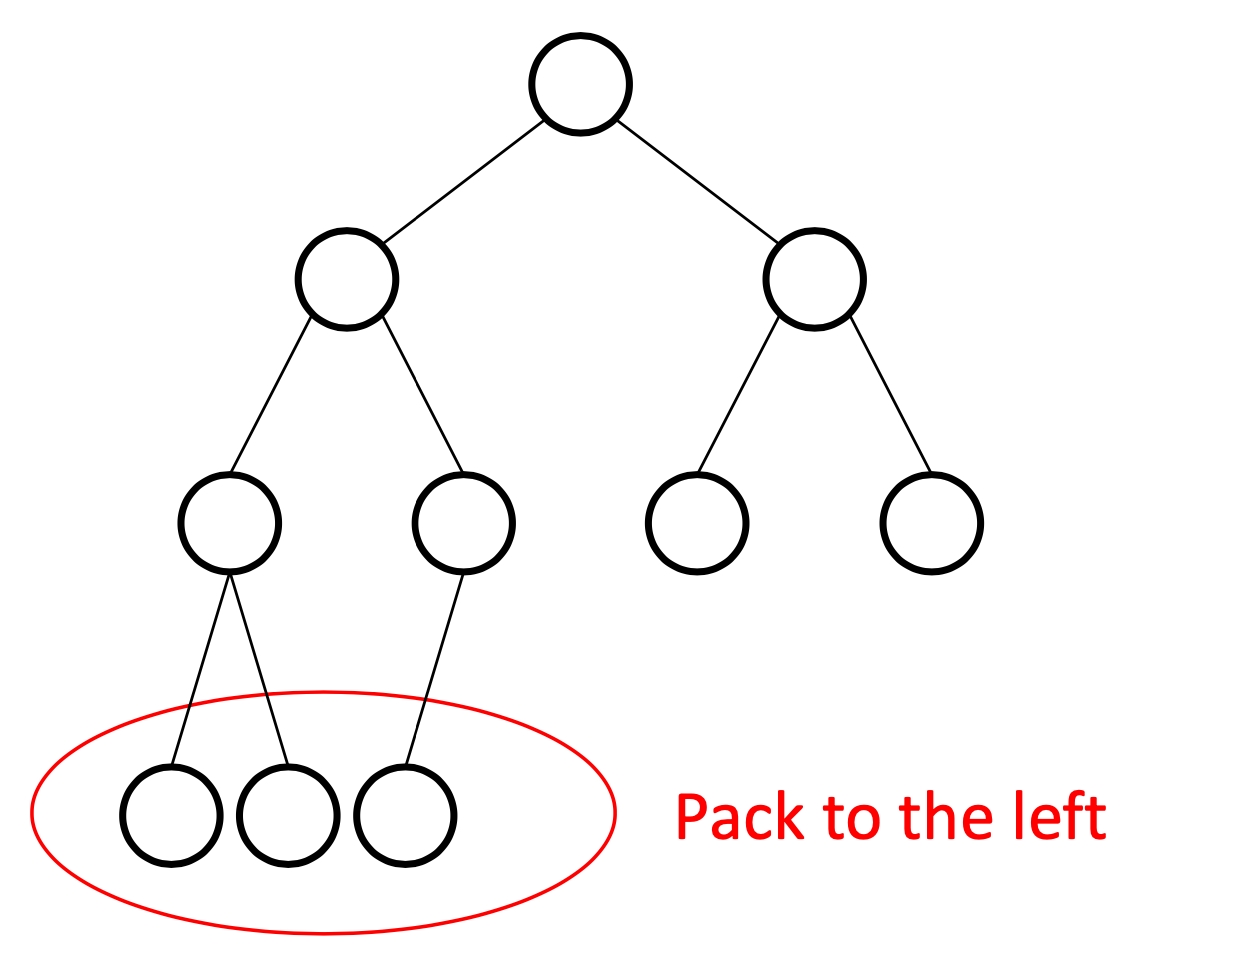
\includegraphics[scale=0.38]{images/05-heap-intro.png}
    \end{figure}

    We also define a special kind of heap called {\bf Min-heap}.
    \begin{definition}
        {\bf Min-heap} is a {\bf heap} in which the value of a node 
        is {\it at least} the value of its parent.
    \end{definition}
    \begin{figure}[htbp]
        \centering
        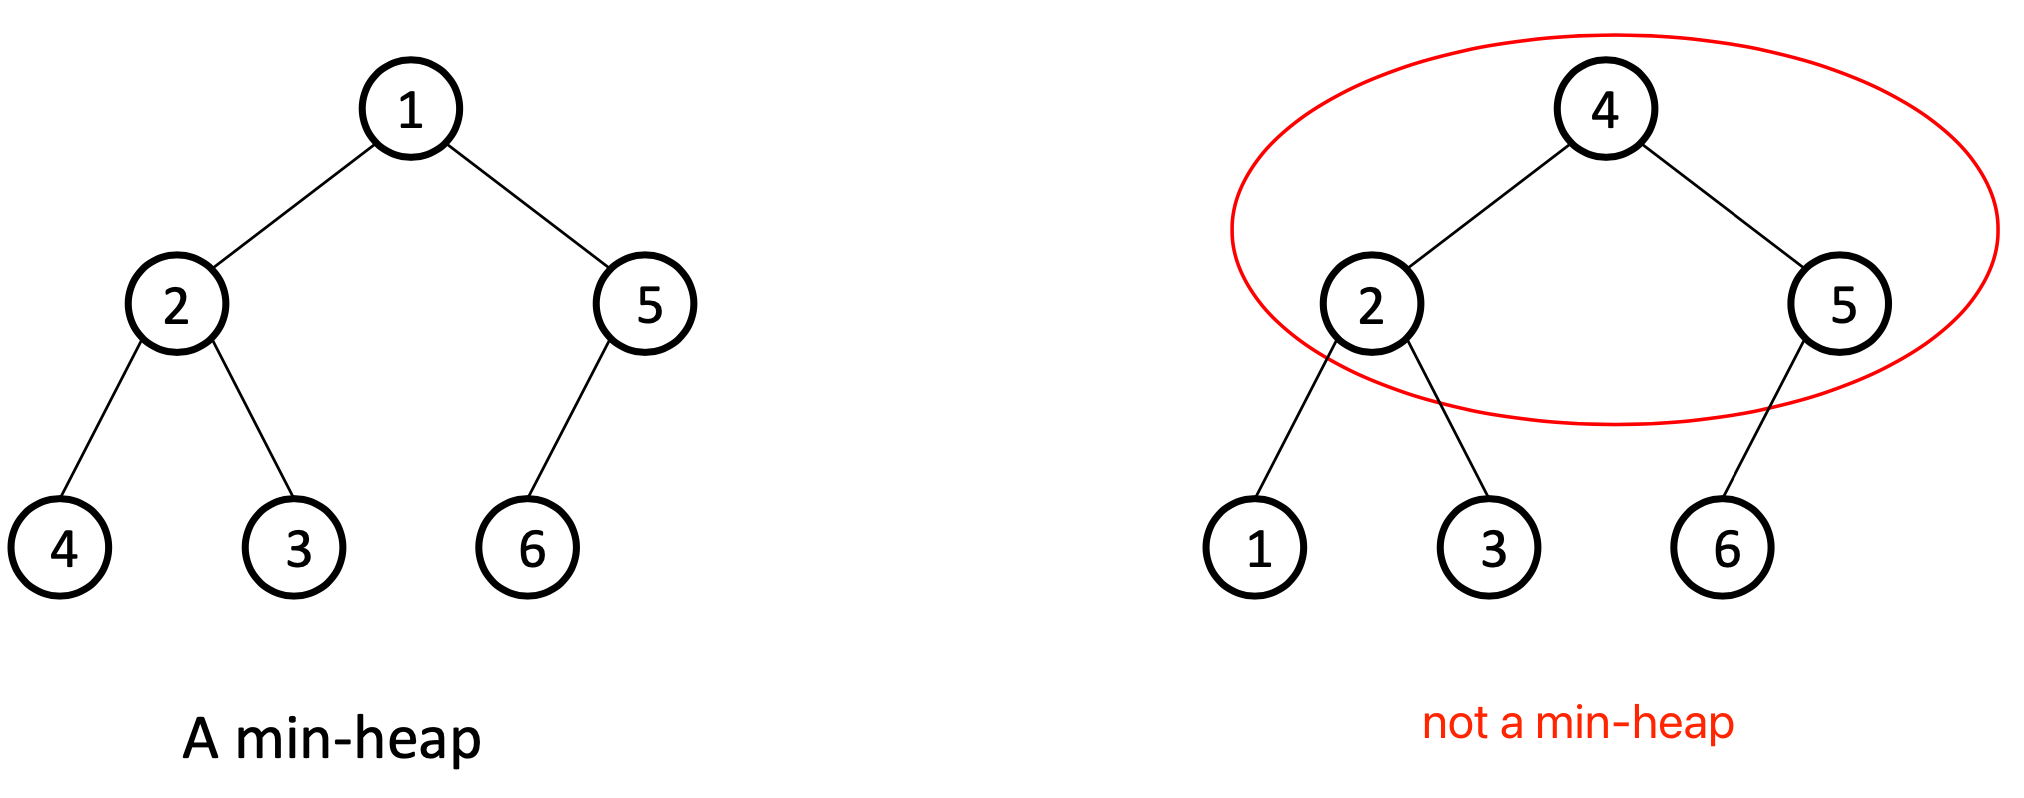
\includegraphics[scale=0.4]{images/05-min-heap-intro.png}
    \end{figure}

    Since {\bf heap} is a special kind of {\bf binary tree}, its height $h$
    and number of elements $n$ are related:
    \begin{theorem}
        For a {\bf heap} with $n$ elements and height $h$, there must be 
        $$2^h\le n<2^{h+1}$$
        thus an $n$-element heap has height $\Theta(\log n)$.
    \end{theorem}
    \begin{proof}
        The proof is trivial, only use the fact that a binary tree with height $h$
        can have at most $2^{h+1}-1$ nodes(height starts from 0), so a heap with 
        height $h$ must have $2^h-1$ nodes before level $h$(since they must be full).
    \end{proof}

    Interestingly, the structure of {\bf heap} is so regular so that we can 
    use an array to represent it.
    \begin{figure}[htbp]
        \centering
        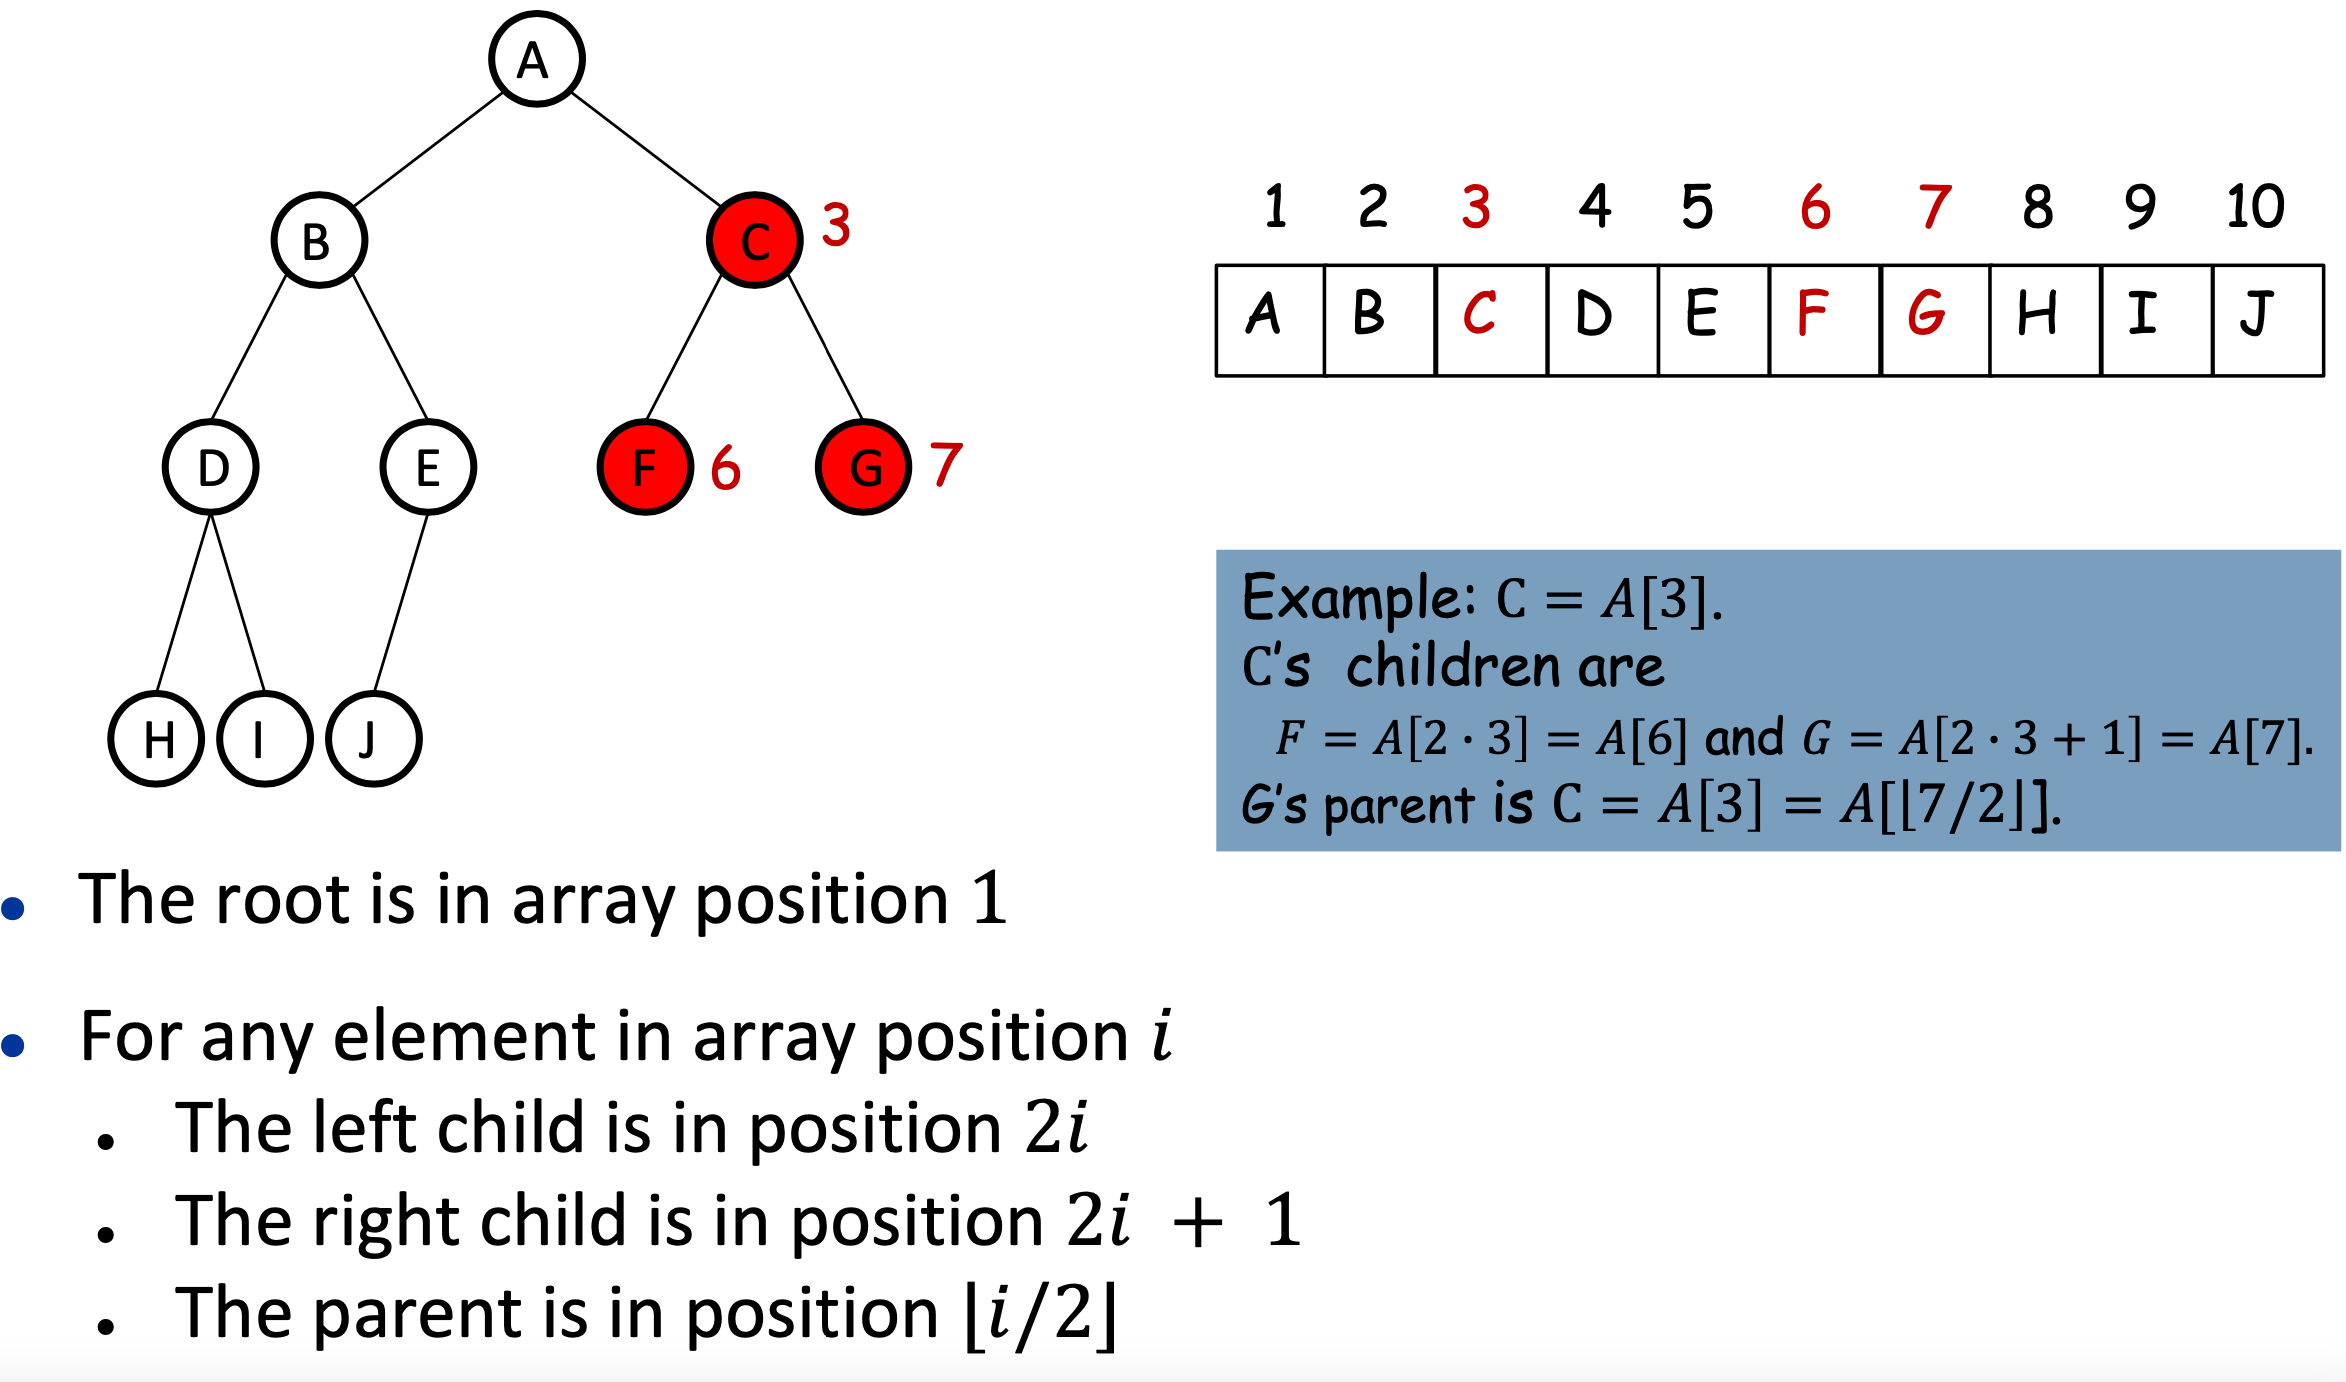
\includegraphics[scale=0.35]{images/05-heap-array.png}
    \end{figure}

    Now with the properties of heap, we can introduce how we can use heap to 
    efficiently perform {\bf insertion} and {\bf extract-min} operations.


    \vspace{0.3in}
    \section{Insertion}

    Recall that a heap must be ``left-packed'', so it is not surprising that 
    if we insert a new node, we should insert it into the {\it next available 
    position at the lowest level}. ``The lowest level'' is because the 
    upper levels are all full, and ``next available'' means the immediate 
    right position of the last node, which allows us to maintain the ``left-packed'' property.

    So if we insert 1 into the heap below, we end up with:
    \begin{figure}[htbp]
        \centering
        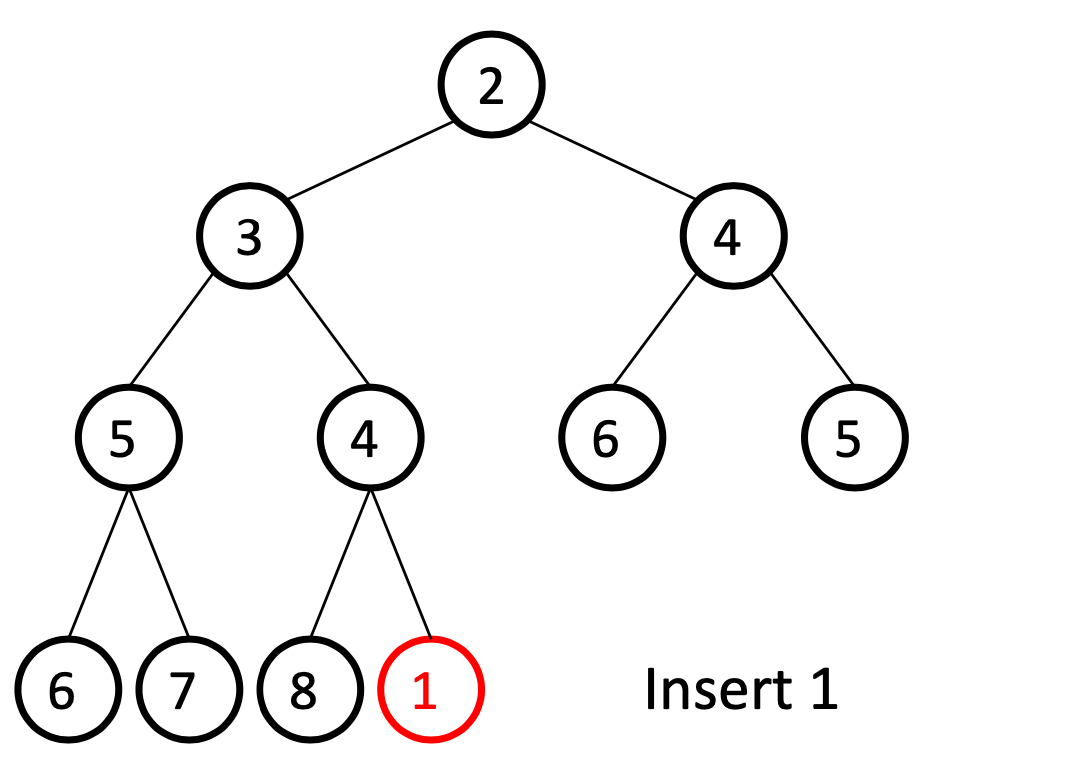
\includegraphics[scale=0.25]{images/05-insert-1.png}
    \end{figure}

    You may have already noticed that the new heap violates the ``min-heap property'', namely
    1 has a parent 4 that is larger than 1. To fix the problem, we consider 
    ``{\bf percolate up(or bubble up)}'': such that if the parent of the node is 
    larger than the node, we swap the parent with that child.

    Here, since $4>1$, we swap parent 4 and its child 1:
    \begin{figure}[htbp]
        \centering
        \qquad 
        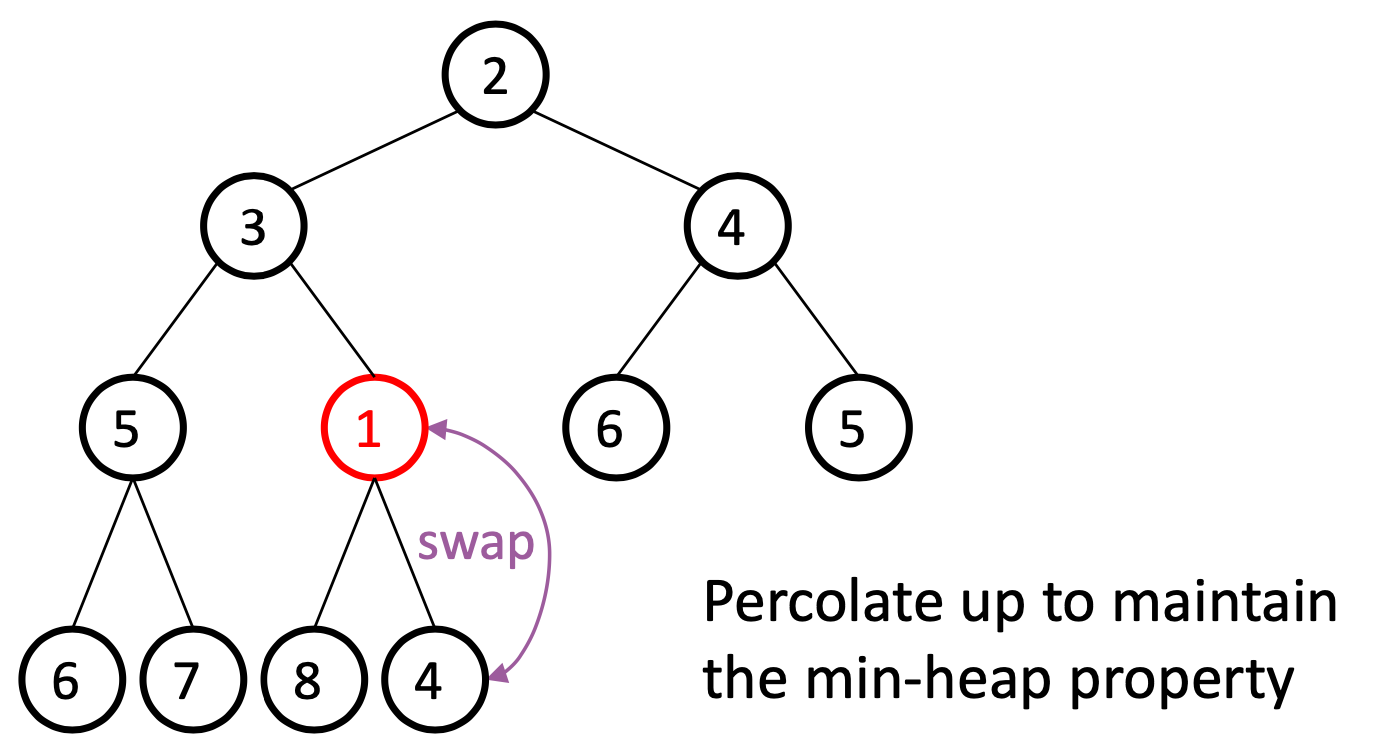
\includegraphics[scale=0.25]{images/05-insert-2.png}
    \end{figure}

    However, 1 still has a parent 3 that larger than 1, so we bubble up again:
    \begin{figure}[htbp]
        \centering
        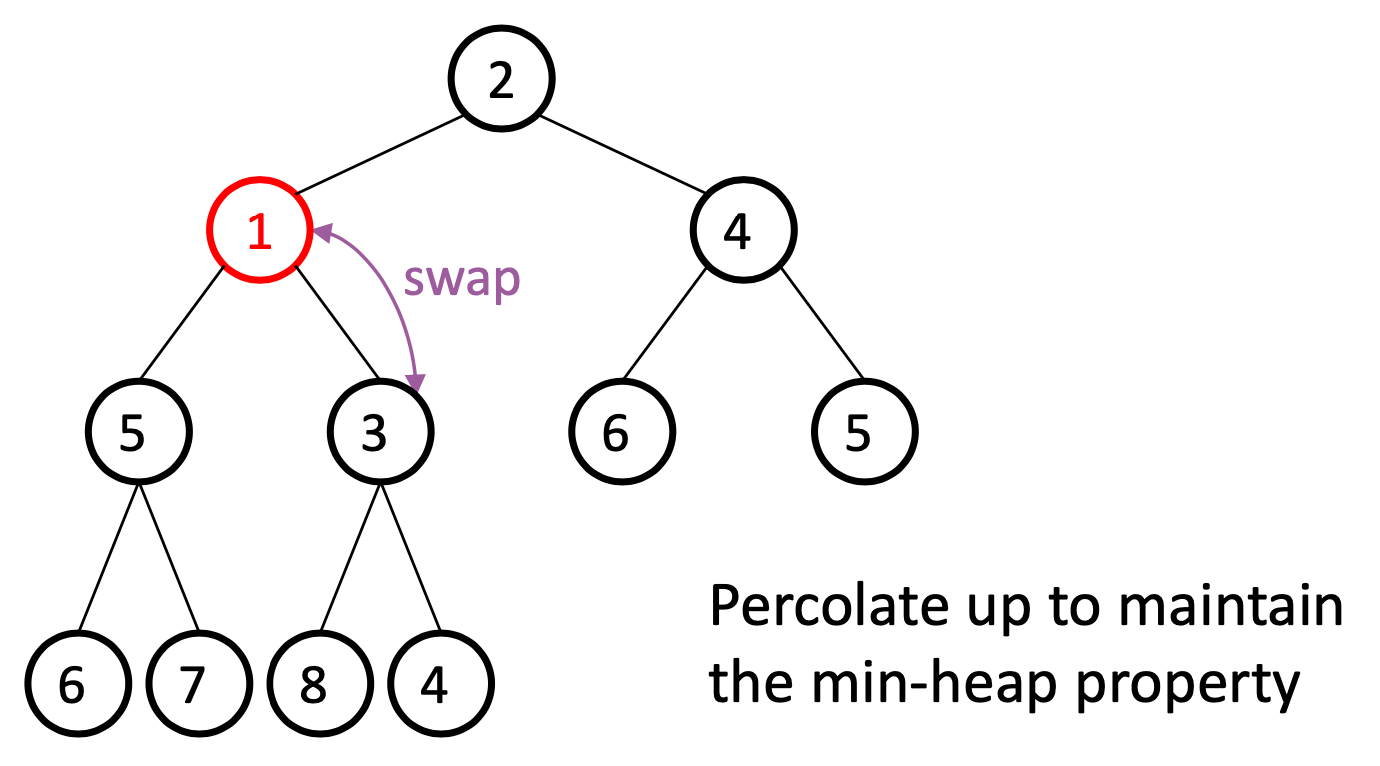
\includegraphics[scale=0.25]{images/05-insert-3.png}
    \end{figure}

    1 still has a parent 2 that larger than 1, bubble up again:
    \begin{figure}[htbp]
        \centering
        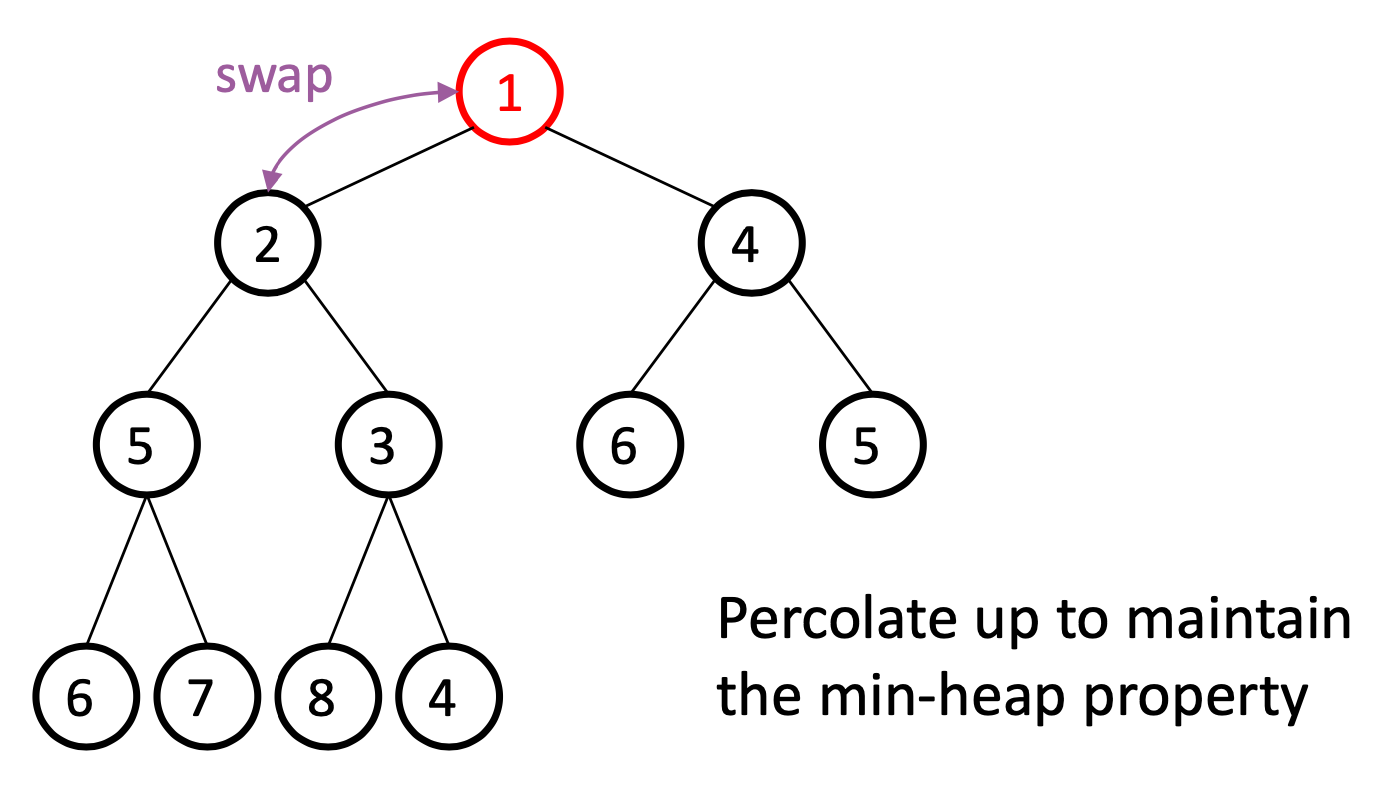
\includegraphics[scale=0.25]{images/05-insert-4.png}
    \end{figure}

    The heap now is fine.

    Since after each swap, the min-heap property is satisfied for the current subtree
    (with the new element as root), so after all those bubble up operations, the 
    min-heap property will certainly be preserved.

    The {\bf time complexity}, which can be measured by number of swaps, is 
    at most the height of heap, i.e., $O(\log n)$.

    We should notice that the swapping process is not necessarily stopped 
    when the new element reaching the top, instead, it stops when 
    its parent is smaller than it. For example, if we insert 2 into the resulted heap above,
    \begin{figure}[htbp]
        \centering
        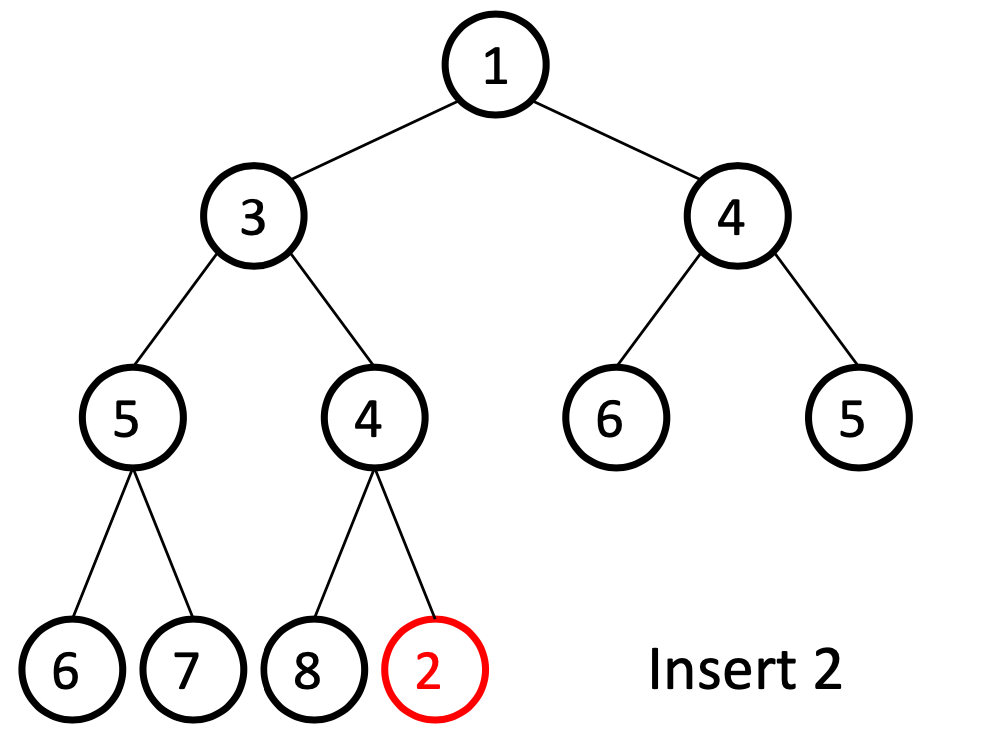
\includegraphics[scale=0.22]{images/05-insert-5.png}\quad 
        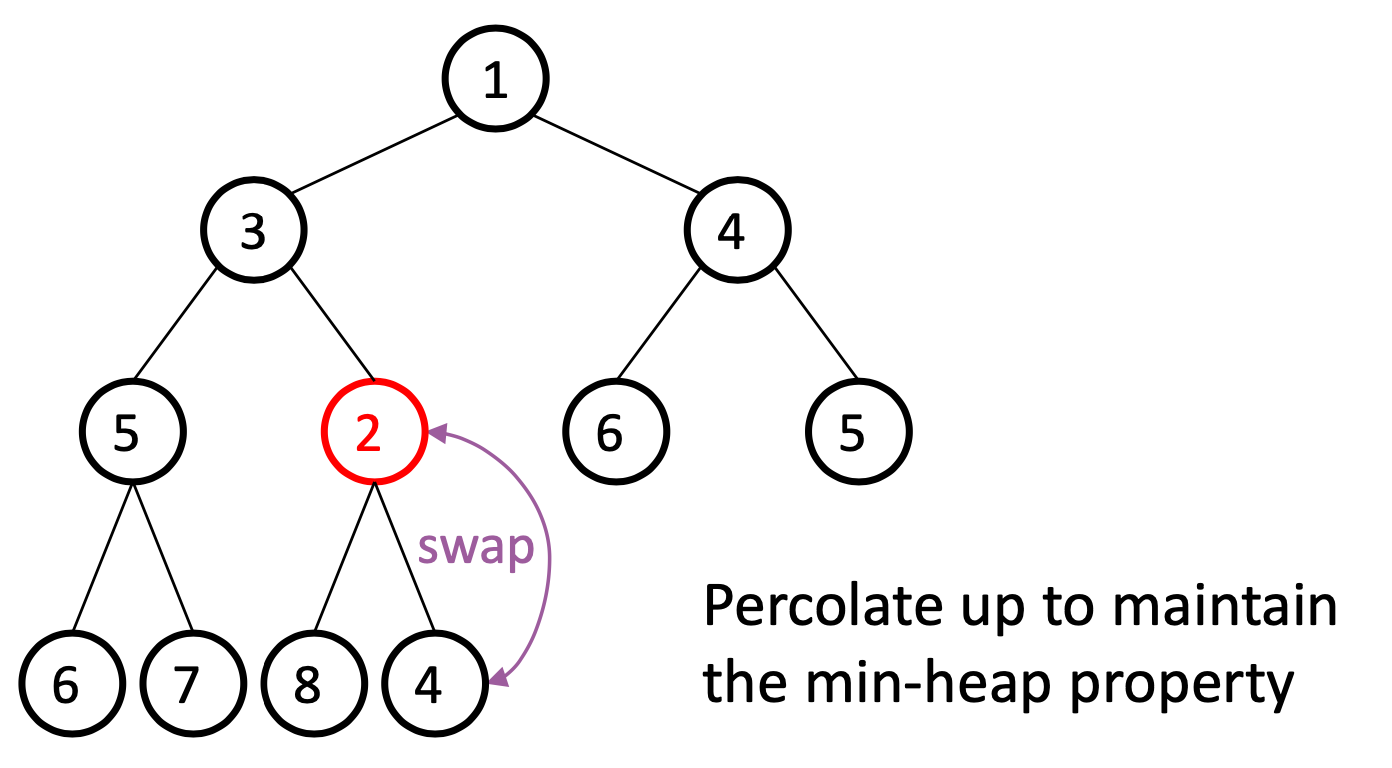
\includegraphics[scale=0.22]{images/05-insert-6.png}\quad 
        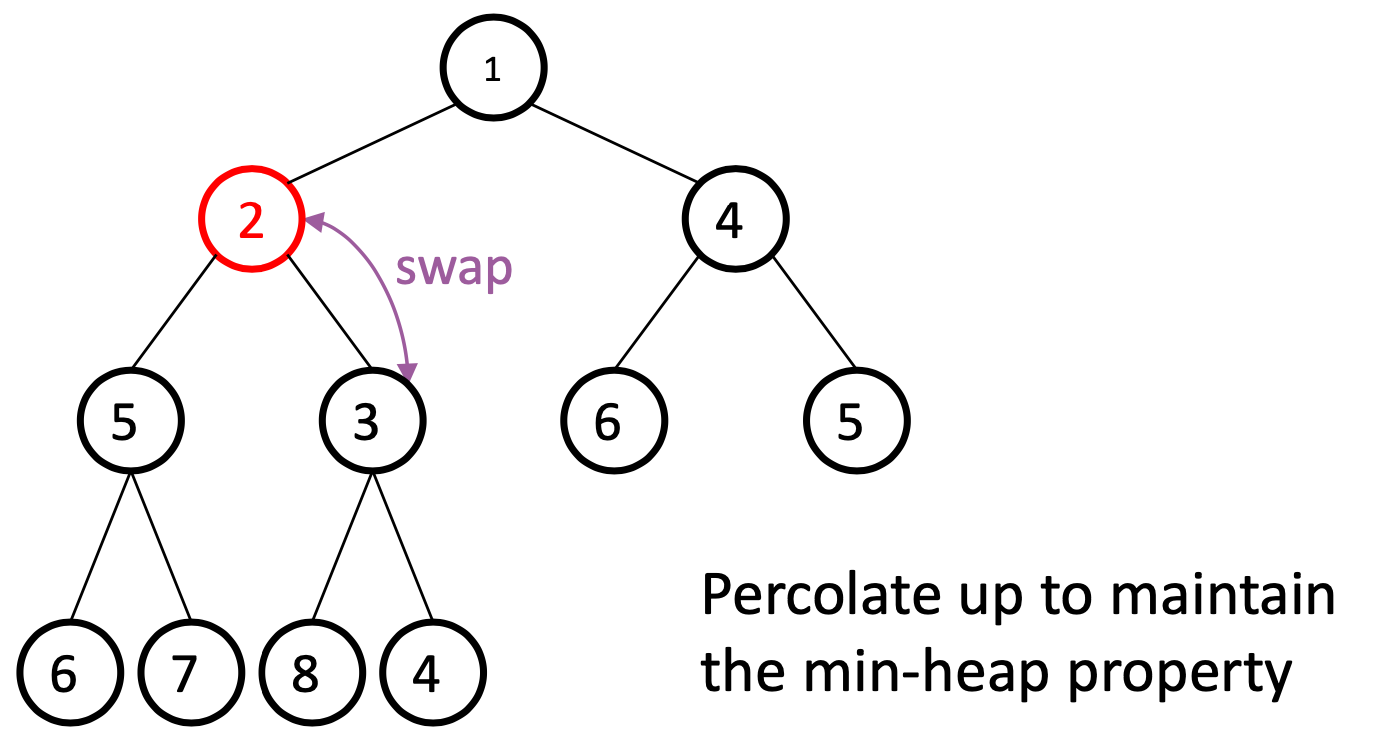
\includegraphics[scale=0.22]{images/05-insert-7.png}\quad 
    \end{figure}
    the process stops before reaching root 1.


    We conclude this section with pseudocode of Insert operation.
    \begin{algorithm*}[htbp]
        \caption{Insert($x$, $i$)}
        \tcp{Insert item $x$ to heap $A[1\cdots i-1]$ creating heap $A[1\cdots i]$}

        $A[i]\lar x$

        $j\lar i$

        \tcp{If smaller than parent, and not reach root yet}
        \While{$A[j]<A\left[\lf \frac{j}{2} \rf\right]$ and $j>1$}{
            \tcp{bubble up $A[j]$, swap with its parent}

            swap $A[j]$ and $A\left[\lf \frac{j}{2} \rf\right]$

            $j=\lf \frac{j}{2} \rf$\qquad \tcp{continue the process on new parent}
        }
    \end{algorithm*}

    \vspace{0.3in}
    \section{Extract-Min}
    
    




\end{spacing}